% 2024年北京高考数学第17题：四棱锥P-ABCD与截面
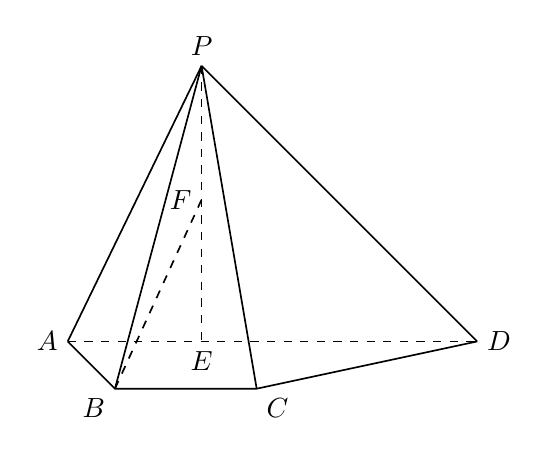
\begin{tikzpicture}[>=stealth,line width=0.6pt,font=\normalsize]
  \coordinate (A) at (0,0);
  \coordinate (B) at (0.6,-0.6);
  \coordinate (C) at (2.4,-0.6);
  \coordinate (D) at (5.2,0);
  \coordinate (P) at (1.7,3.5);
  \coordinate (E) at (1.7,0);
  \coordinate (F) at (1.7,1.8);

  % 实线可见边
  \draw (A) -- (B) -- (C) -- (D);
  \draw (P) -- (A);
  \draw (P) -- (B);
  \draw (P) -- (C);
  \draw (P) -- (D);

  % 虚线不可见底边与内部线
  \draw[dashed] (A) -- (D);
  \draw[dashed] (P) -- (E);
  \draw[dashed] (B) -- (F);

  % 顶点标注
  \node[above] at (P) {$P$};
  \node[left] at (A) {$A$};
  \node[below left] at (B) {$B$};
  \node[below right] at (C) {$C$};
  \node[right] at (D) {$D$};
  \node[below] at (E) {$E$};
  \node[left] at (F) {$F$};
\end{tikzpicture}
